% Provenance (never printed): see sources/outline_sources.md (Year 3: rift
% models, normal-fault systems, metamorphic core complexes, strike-slip
% systems). Brief: sources/book5/BRIEFS.md, ch. 9. Curves from
% figdata/bachelor-3/domino_extension.py and rollover.py. Exercise and problem
% values in the Book 5 scratch calculator calc/ch09.py.
\chapter{Tektonik Ekstensi dan Sesar Geser-Mendatar}\label{ch:b3:extension-strike-slip}

Di antara Sierra Nevada dan Dataran Tinggi Colorado, pegunungan dan cekungan
berselang-seling seperti alur bajakan di ladang, tiap pegunungan ialah blok kerak yang miring
sepanjang sesar normal. Di inti beberapa pegunungan ini, batuan yang dahulu
terkubur sedalam 23 sampai \qty{30}{km}, pada suhu 500 sampai \qty{650}{\celsius}, kini
tersingkap di permukaan, di bawah satu sesar yang hanya miring beberapa derajat. Suatu benua dapat
ditarik berpisah dengan faktor dua atau lebih, dan terkoyak ke samping sepanjang sesar
yang membengkok, bertingkat, dan membuka cekungan sedalam \qty{10}{km}. Bab ini membangun
geometri perpanjangan dan sesar geser-mendatar, beberapa kaidah yang
mengaturnya, serta bukti yang ditinggalkan sistem nyata.
% ledger: cooper10:snake-range, mcq05:basin-range, tb93:dead-sea-basin

\begin{recall}
Sesar normal, sesar geser-mendatar, dan sesar transform, paruh-graben, serta
celah benua dibahas di volume Tahun 1, pada bab tentang celah dan tentang sesar, lipatan
dan fabrik, beserta teori Anderson: dengan $\sigma_1$ vertikal, sesar normal
berkemiringan $\ang{45} + \phi/2$, sekitar \ang{60}; dengan $\sigma_2$ vertikal, sesar geser-mendatar
berjurus pada $\ang{45} - \phi/2$ dari $\sigma_1$. Hukum Byerlee tentang gesekan batuan,
$\tau = 0.85\,\sigma_n$ di bawah \qty{200}{MPa} dan $\tau =
\qty{50}{MPa} + 0.6\,\sigma_n$ di atasnya, terdapat di bab tentang tegangan, regangan, dan
reologi. Model peregangan, yang menipiskan litosfer secara seragam
dengan faktor $\beta$, serta cekungan celah, ada di volume Tahun 2, pada babnya
yang membandingkan cekungan sedimen. \omterm{def:b3:deformation-mechanisms:shear-zone}{Zona geser} dan milonit dibahas dalam
\cref{ch:b3:deformation-mechanisms}; kedalaman ke \omterm{def:b3:extension-strike-slip:detachment}{sesar detasemen} dari luas berlebih
$A = Sh$, yang dijelaskan dalam \cref{ch:b3:structural-analysis}.
\end{recall}
% ledger: byerlee:1975

\section{Dua model celah}\label{sec:b3:extension-strike-slip:models}

Model peregangan di volume Tahun 2 menipiskan seluruh litosfer dengan
faktor yang sama di bawah tempat yang sama: kerak dan mantel menipis bersama,
secara simetris, oleh geser murni. Banyak tepi celah tidak simetris: satu sisi
berupa wilayah luas blok yang miring, sisi lainnya lereng sempit yang curam, dan
penipisan mantel terletak di samping, bukan di bawah, penipisan kerak.

\begin{definition}[Model celah geser sederhana]\label{def:b3:extension-strike-slip:rift-models}
Pada \emph{model celah geser sederhana}\index{model celah geser sederhana}, litosfer
ditarik berpisah sepanjang \omterm{def:b3:deformation-mechanisms:shear-zone}{zona geser} sudut rendah yang memotong litosfer dari
permukaan hingga dasarnya. Lempeng di atas \omterm{def:b3:deformation-mechanisms:shear-zone}{zona geser}, yaitu lempeng atas,
kehilangan bagian bawahnya; lempeng di bawah, yaitu lempeng bawah, tertarik keluar
dari bawahnya. Penipisan kerak dan penipisan mantel
bergeser ke samping, serta kedua tepi konjugat yang terbentuk saat benua
pecah bersifat asimetris.
\end{definition}

Celah nyata memadukan keduanya: pensesaran rapuh di kerak atas, penipisan duktil
di bawahnya, serta mantel yang mungkin menipis di wilayah yang lebih luas atau lebih sempit daripada
kerak (peregangan bergantung kedalaman). Di mana mantel panas naik di bawah
celah, atau di bawah sisinya pada kasus geser sederhana, daya apung mengangkat
bahu celah, yang berdiri sebagai gunung di atas dasar cekungan.

\begin{omfigure}
\begin{tikzpicture}[scale=0.95, >=stealth]
% (a) pure shear
\begin{scope}
\fill[omLithBasalt!40] (0,-3.2) rectangle (6.6,-1.3);
\fill[omLithGranite!50] (0,0) -- (2.2,0) -- (2.5,-0.35) -- (4.1,-0.35) -- (4.4,0) -- (6.6,0) -- (6.6,-1.3)
  -- (4.4,-1.3) -- (3.3,-0.95) -- (2.2,-1.3) -- (0,-1.3) -- cycle;
\fill[omLithBasalt!40] (2.2,-1.3) -- (3.3,-0.95) -- (4.4,-1.3) -- cycle;
\fill[orange!25] (0,-3.2) -- (1.8,-3.2) -- (3.3,-2.1) -- (4.8,-3.2) -- (6.6,-3.2) -- (6.6,-3.7) -- (0,-3.7) -- cycle;
\draw (0,0) -- (2.2,0) -- (2.5,-0.35) -- (4.1,-0.35) -- (4.4,0) -- (6.6,0);
\draw (0,-1.3) -- (2.2,-1.3) -- (3.3,-0.95) -- (4.4,-1.3) -- (6.6,-1.3);
\draw (0,-3.2) -- (1.8,-3.2) -- (3.3,-2.1) -- (4.8,-3.2) -- (6.6,-3.2);
\draw[thick] (2.2,0) -- (2.75,-0.85); \draw[thick] (4.4,0) -- (3.85,-0.85);
\node[font=\scriptsize] at (0.7,-0.65) {kerak};
\node[font=\scriptsize, align=center] at (0.9,-2.25) {mantel\\ litosfer};
\node[font=\scriptsize] at (1.2,-3.48) {astenosfer};
\draw[<-] (-0.1,0.25) -- (0.6,0.25); \draw[->] (6.0,0.25) -- (6.7,0.25);
\node[font=\small] at (3.3,-4.2) {(a) geser murni};
\end{scope}
% (b) simple shear: crust thinned near the breakaway (left), mantle beneath the upper plate (right)
\begin{scope}[xshift=7.4cm]
\fill[omLithBasalt!40] (0,-3.2) rectangle (6.6,-1.3);
\fill[omLithGranite!50] (0,0) -- (0.9,0) -- (1.2,-0.3) -- (2.2,-0.3) -- (2.5,0) -- (4.0,0)
  .. controls (4.6,0.18) and (5.2,0.18) .. (5.8,0) -- (6.6,0) -- (6.6,-1.3)
  -- (2.9,-1.3) -- (2.0,-0.7) -- (1.2,-1.3) -- (0,-1.3) -- cycle;
\fill[omLithBasalt!40] (1.2,-1.3) -- (2.0,-0.7) -- (2.9,-1.3) -- cycle;
\fill[orange!25] (0,-3.2) -- (3.4,-3.2) -- (4.8,-2.1) -- (6.0,-3.2) -- (6.6,-3.2) -- (6.6,-3.7) -- (0,-3.7) -- cycle;
\draw (0,0) -- (0.9,0) -- (1.2,-0.3) -- (2.2,-0.3) -- (2.5,0) -- (4.0,0)
  .. controls (4.6,0.18) and (5.2,0.18) .. (5.8,0) -- (6.6,0);
\draw (0,-1.3) -- (1.2,-1.3) -- (2.0,-0.7) -- (2.9,-1.3) -- (6.6,-1.3);
\draw (0,-3.2) -- (3.4,-3.2) -- (4.8,-2.1) -- (6.0,-3.2) -- (6.6,-3.2);
\draw[omThm, very thick] (0.9,0) .. controls (2.4,-0.9) and (3.9,-1.8) .. (5.4,-3.2);
\node[font=\scriptsize, align=center] at (5.0,-0.6) {lempeng atas};
\node[font=\scriptsize, align=center] at (1.3,-2.3) {lempeng bawah};
\node[omThm, font=\scriptsize, align=center] at (3.0,-2.15) {zona\\ geser};
\node[font=\scriptsize, align=center] at (4.9,0.42) {sisi terangkat};
\draw[<-] (-0.1,0.25) -- (0.6,0.25); \draw[->] (6.0,0.25) -- (6.7,0.25);
\node[font=\small] at (3.3,-4.2) {(b) geser sederhana};
\end{scope}
\end{tikzpicture}

\par\smallskip{\small Dua model ekstrem sebuah celah (tidak sesuai skala). (a) Geser
murni: kerak dan litosfer mantel menipis bersama di bawah celah, dengan sesar normal
di kedua sisi. (b) Geser sederhana: \omterm{def:b3:deformation-mechanisms:shear-zone}{zona geser} sudut rendah memotong
litosfer; kerak menipis dekat jejak permukaannya, mantel di bawah
sisi seberang, di bawah lempeng atas, sehingga celah asimetris dan sisinya
di atas mantel yang menipis terangkat.}\label{fig:b3:extension-strike-slip:models}
\end{omfigure}

\section{Sistem sesar normal}\label{sec:b3:extension-strike-slip:faults}

\begin{definition}[Pensesaran domino]\label{def:b3:extension-strike-slip:domino}
Dalam \emph{pensesaran domino}\index{pensesaran domino}, sekumpulan sesar normal planar sejajar
memotong kerak atas menjadi blok-blok kaku yang, seiring wilayah itu meregang,
berputar bersama seperti deretan buku yang roboh: sesarnya menjadi
lebih landai, dan lapisan yang semula mendatar kini miring ke arah sebaliknya.
\end{definition}

\begin{theorem}[Perluasan oleh domino]\label{thm:b3:extension-strike-slip:domino}
Misalkan blok-blok kaku yang dibatasi oleh sesar planar sejajar yang mula-mula memiliki kemiringan
$\theta_0$ berotasi hingga sesarnya memiliki kemiringan $\theta$. Lapisan kemudian memiliki kemiringan $\theta_0
- \theta$, menjauhi sesar, dan wilayah tersebut telah meregang oleh
faktor
\[
  \beta = \frac{\sin\theta_0}{\sin\theta} .
\]
\end{theorem}

\begin{proof}
Blok-blok itu kaku, sehingga jarak tegak lurus $d$ antara dua
sesar yang bersebelahan tidak berubah. Sepanjang garis horizontal, dua bidang sejajar
yang memiliki kemiringan $\theta$ dan berjarak $d$ memotong ruas sepanjang $d/\sin
\theta$; lebar wilayah sebanding dengan panjang ruas itu, dari
$d/\sin\theta_0$ menjadi $d/\sin\theta$. Blok-blok berputar sebesar sudut
yang dengannya sesar telah melandai, yakni $\theta_0 - \theta$, dan lapisan, yang mula-mula mendatar,
ikut berputar bersama blok-blok itu.
\end{proof}

Rotasi saja hanya memberikan perluasan kecil: sesar yang mula-mula bersudut \ang{60} dan
melandai hingga \ang{30} memperluas wilayah sebesar $\beta = 1.73$. Blok-blok itu tidak dapat berotasi
terus tanpa batas: sebuah sesar makin sulit tergelincir ketika makin landai, karena $\sigma_1$ vertikal
menekannya lebih kuat dan menggesernya lebih sedikit.

\begin{proposition}[Penguncian gesekan sesar normal]\label{prop:b3:extension-strike-slip:lockup}
Misalkan sebuah sesar tanpa kohesi dengan koefisien gesek $\mu$ membentuk sudut
$t$ terhadap $\sigma_1$, dengan semua tegangan efektif. Sesar tergelincir ketika \omterm{def:b3:structural-analysis:palaeostress}{rasio
tegangan} utama mencapai
\[
  \frac{\sigma_1}{\sigma_3} = \frac{1 + \mu\cot t}{1 - \mu\tan t} ,
\]
yang nilainya paling kecil, $(\sqrt{1 + \mu^2} + \mu)^2$, pada $\tan2t = 1/\mu$, dan
tak hingga pada $\tan t = 1/\mu$. Dengan $\sigma_1$ vertikal, kemiringan sesarnya adalah
$\ang{90} - t$: sesar normal yang kemiringannya kurang dari $\arctan\mu$ tidak dapat tergelincir
sama sekali.
\end{proposition}

\begin{proof}
Tulis $m = (\sigma_1 + \sigma_3)/2$ dan $s = (\sigma_1 - \sigma_3)/2$. Pada
bidang, $\sigma_n = \sigma_1\sin^2t + \sigma_3\cos^2t = m - s\cos2t$ dan
$\tau = (\sigma_1 - \sigma_3)\sin t\cos t = s\sin2t$. Tergelincir memerlukan $\tau =
\mu\sigma_n$; dengan membagi dengan $\sigma_3\sin t\cos t$ dan mengumpulkan $\sigma_1$
menghasilkan rasionya, yang penyebutnya nol pada $\tan t = 1/\mu$. Dalam bentuk lain,
syaratnya berbunyi $s(\sin2t + \mu\cos2t) = \mu m$. Kurung ini paling
besar $\sqrt{1 + \mu^2}$, dicapai pada $\tan2t = 1/\mu$, saat tergelincir memerlukan
nilai terkecil $s/m = \mu/\sqrt{1 + \mu^2}$; lalu $\sigma_1/\sigma_3 = (m + s)/(m - s) =
(\sqrt{1 + \mu^2} + \mu)/(\sqrt{1 + \mu^2} - \mu) = (\sqrt{1 + \mu^2} +
\mu)^2$, karena hasil kali dua kurung terakhir bernilai 1.
\end{proof}

Dengan $\mu = 0.6$ menurut Byerlee, sesar normal dengan orientasi paling menguntungkan memiliki kemiringan \ang{60.5} dan
tergelincir ketika $\sigma_1 = 3.12\,\sigma_3$, sesar pada \ang{45} memerlukan $4.0$, dan
tidak ada sesar yang kemiringannya kurang dari \ang{31} dapat tergelincir; dengan $\mu = 0.85$ kemiringan penguncian adalah
\ang{40}. Gambar di bawah memperlihatkan kedua hasil itu. Ketika sekumpulan domino mendekati
penguncian, sekumpulan sesar curam baru memotong yang lama: wilayah yang sangat meregang
memperlihatkan beberapa generasi sesar.

\begin{omfigure}
\begin{tikzpicture}
\begin{groupplot}[group style={group size=2 by 1, horizontal sep=1.6cm},
  omrecord, width=0.47\linewidth, height=0.42\linewidth, title style={font=\small},
  legend style={font=\scriptsize, legend cell align=left}]
\nextgroupplot[title={(a) perluasan oleh domino kaku}, xlabel={kemiringan sesar saat ini $\theta$ (\unit{\degree})},
  ylabel={faktor perluasan $\beta$}, xmin=10, xmax=70, ymin=1, ymax=4,
  legend style={at={(0.97,0.97)}, anchor=north east}]
% computed in figdata/bachelor-3/domino_extension.py
\addplot[omDef, thick] table[x=dip, y=b70] {figdata/out/bachelor-3-domino_extension-beta.dat};
\addlegendentry{$\theta_0 = \ang{70}$}
\addplot[red!70!black, thick, densely dashed] table[x=dip, y=b60] {figdata/out/bachelor-3-domino_extension-beta.dat};
\addlegendentry{$\theta_0 = \ang{60}$}
\addplot[black, thick, densely dotted] table[x=dip, y=b45] {figdata/out/bachelor-3-domino_extension-beta.dat};
\addlegendentry{$\theta_0 = \ang{45}$}
\nextgroupplot[title={(b) rasio tegangan yang diperlukan untuk tergelincir}, xlabel={kemiringan sesar (\unit{\degree})},
  ylabel={$\sigma_1/\sigma_3$}, xmin=20, xmax=90, ymode=log, ymin=1, ymax=40,
  log ticks with fixed point, ytick={1,2,5,10,20,40},
  legend style={at={(0.97,0.97)}, anchor=north east}]
\addplot[omDef, thick] table[x=dip, y=r060] {figdata/out/bachelor-3-domino_extension-lockup.dat};
\addlegendentry{$\mu = 0.6$}
\addplot[red!70!black, thick, densely dashed] table[x=dip, y=r085] {figdata/out/bachelor-3-domino_extension-lockup.dat};
\addlegendentry{$\mu = 0.85$}
\end{groupplot}
\end{tikzpicture}

\par\smallskip{\small (a) Faktor perluasan suatu wilayah domino kaku saat
sesarnya berotasi dari kemiringan awal $\theta_0$ menjadi $\theta$. (b) \omterm{def:b3:structural-analysis:palaeostress}{Rasio
tegangan} utama efektif yang diperlukan untuk menggeser sesar normal dengan kemiringan tertentu
di bawah $\sigma_1$ vertikal, untuk dua koefisien gesek menurut Byerlee: paling kecil
dekat \ang{60} dan \ang{65}, tak hingga pada kemiringan penguncian \ang{31} dan
\ang{40}.}\label{fig:b3:extension-strike-slip:domino}
\end{omfigure}

Banyak sesar normal besar yang melengkung, curam di permukaan dan melandai di
kedalaman menjadi sesar atau \omterm{def:b3:deformation-mechanisms:shear-zone}{zona geser} yang hampir mendatar.

\begin{definition}[Sesar detasemen, sesar listrik, antiklin rollover]\label{def:b3:extension-strike-slip:detachment}
Yang disebut \emph{sesar detasemen}\index{sesar detasemen} adalah sesar normal bersudut rendah
atau \omterm{def:b3:deformation-mechanisms:shear-zone}{zona geser} dengan pergeseran besar, kilometer hingga puluhan kilometer, yang
memisahkan lempeng atas yang meregang dari lempeng bawah yang terdeformasi secara berbeda. Yang
disebut \emph{sesar listrik}\index{sesar listrik} adalah sesar normal yang kemiringannya
berkurang seiring kedalaman, profilnya cekung ke atas. Ketika dinding gantung dari
sesar listrik bergerak turun dan menjauh, dinding itu melengkung agar tetap bersentuhan dengan
sesar: lapisannya miring ke arah sesar membentuk lipatan lebar, yang disebut \emph{antiklin
rollover}\index{antiklin rollover}.
\end{definition}

\begin{method}[Konstruksi lompatan horizontal konstan]\label{met:b3:extension-strike-slip:heave}
Untuk menggambar dinding gantung dari \omterm{def:b3:extension-strike-slip:detachment}{sesar listrik} setelah pergeseran horizontal
$H$, yakni lompatan horizontal, pada penampang sejajar dengan arah pergeseran:
\begin{enumerate}
  \item Bagi dinding gantung menjadi kolom-kolom vertikal. Geser setiap kolom
        ke samping sejauh $H$, menjauhi dinding bawah.
  \item Turunkan setiap kolom sebesar penurunan sesar di bawahnya: kolom yang
        mulai di tempat sesar berada pada kedalaman $f(x)$ dan berakhir di tempat ia berada
        pada $f(x + H)$ turun sebesar $f(x + H) - f(x)$, sehingga alasnya
        kembali menempel pada sesar.
  \item Ruang yang tersisa di antara dinding bawah dan dinding gantung yang telah digeser adalah
        paruh-graben, yang terisi seiring terbukanya oleh sedimen yang menebal ke arah
        sesar.
\end{enumerate}
Dibaca mundur, konstruksi ini memulihkan penampang dan memprediksi bentuk
sesar dari bentuk \omterm{def:b3:extension-strike-slip:detachment}{antiklin rollover}.
\end{method}

Luas di bawah level awal sebuah lapisan, diukur dari sesar, adalah
luas pada \cref{ch:b3:structural-analysis} dengan tanda dibalik: $A =
H(D - z_0)$ untuk lapisan yang mula-mula berada pada kedalaman $z_0$ di atas \omterm{def:b3:extension-strike-slip:detachment}{sesar detasemen} pada
kedalaman $D$, karena batuan di bawah lapisan itu mempertahankan luasnya sementara panjangnya bertambah
sebesar $H$. Pengukuran $A$ dan $H$ pada penampang seismik memberikan kedalaman
detasemen. Gambar di bawah ini memperlihatkan konstruksinya.

\begin{omfigure}
\begin{tikzpicture}
\begin{axis}[width=0.9\linewidth, height=0.36\linewidth, omsection,
  xmin=-2, xmax=24, ymin=0, ymax=6, y dir=reverse,
  xlabel={jarak (\unit{km})}, ylabel={kedalaman (\unit{km})},
  legend style={font=\scriptsize, legend cell align=left, at={(0.98,0.27)}, anchor=south east}]
% computed in figdata/bachelor-3/rollover.py (heave 2 km, detachment at 5 km)
\addplot[name path=fault, black, very thick] table[x=x, y=z] {figdata/out/bachelor-3-rollover-fault.dat};
\addlegendentry{sesar listrik}
\addplot[name path=top, omDef, thick] table[x=x, y=z] {figdata/out/bachelor-3-rollover-top.dat};
\addlegendentry{puncak dinding gantung}
\addplot[omDef, thick, densely dashed] table[x=x, y=z] {figdata/out/bachelor-3-rollover-bed.dat};
\addlegendentry{lapisan mula-mula pada \qty{2}{km}}
\addplot[gray, dashed, forget plot] coordinates {(-2,0) (24,0)};
\addplot[gray, dashed, forget plot] coordinates {(-2,5) (24,5)};
\node[font=\scriptsize, anchor=west] at (axis cs:15,5.35) {detasemen};
\node[font=\scriptsize] at (axis cs:3.9,0.45) {paruh-graben};
\node[font=\scriptsize] at (axis cs:-1,1.5) {dinding bawah};
\node[font=\scriptsize] at (axis cs:9.5,1.15) {antiklin rollover};
\end{axis}
\end{tikzpicture}

\par\smallskip{\small \omterm{def:b3:extension-strike-slip:detachment}{Sesar listrik} dengan kemiringan \ang{60} di permukaan dan
melandai menjadi detasemen pada \qty{5}{km}, setelah lompatan horizontal \qty{2}{km}
yang digambar dengan konstruksi lompatan konstan. Puncak dinding gantung dan sebuah lapisan
yang lebih dalam melengkung ke arah sesar membentuk rollover; luas di bawah
puncak awal, \qty{10}{km^2}, sama dengan lompatan horizontal dikali kedalaman detasemen, dan di bawah
lapisan yang lebih dalam \qty{6}{km^2}, yaitu lompatan horizontal dikali tingginya di atas lapisan itu.}\label{fig:b3:extension-strike-slip:rollover}
\end{omfigure}

Sesar normal tidak berlangsung tanpa batas. Di tempat satu sesar habis sepanjang jurus,
perpindahannya beralih ke sesar lain, yang sering memiliki kemiringan ke arah sebaliknya, dan
paruh-graben dari sebuah celah bergantian polaritasnya di sepanjang celah tersebut.

\begin{definition}[Zona transfer]\label{def:b3:extension-strike-slip:transfer}
Yang disebut \emph{zona transfer}\index{zona transfer} adalah daerah di antara dua
segmen sesar normal atau segmen celah yang tumpang tindih atau bergeser, tempat perpanjangan
berpindah dari satu ke yang lain: tanjakan relai di antara dua sesar
dengan polaritas yang sama, tinggian di antara paruh-graben dengan polaritas berlawanan, atau sebuah
sesar geser-mendatar, yaitu sesar transfer, yang sejajar dengan perpanjangan.
\end{definition}

\section{Kompleks inti metamorf}\label{sec:b3:extension-strike-slip:core}

\begin{definition}[Kompleks inti metamorf, engsel bergulir]\label{def:b3:extension-strike-slip:core-complex}
Yang disebut \emph{kompleks inti metamorf}\index{kompleks inti metamorf} adalah kubah
batuan metamorf dan milonit yang terangkat dari kerak tengah atau bawah,
di bawah \omterm{def:b3:extension-strike-slip:detachment}{sesar detasemen} yang plat atasnya berupa mosaik blok miring
batuan kerak atas. Dalam model \emph{engsel bergulir}\index{engsel bergulir},
detasemen tergelincir dengan kemiringan sedang di kedalaman; ketika plat atas
bergerak menjauh, dinding bawah yang tidak lagi terbebani terangkat secara isostasi dan melengkung,
sehingga setiap bagian sesar terputar hingga kemiringan rendah dan berhenti tergelincir setelah melewati
engsel yang berpindah bersama perpanjangan.
\end{definition}

Milonit di dinding bawah merekam bagian terdalam dari kisah ini: milonit tersebut adalah
\omterm{def:b3:deformation-mechanisms:shear-zone}{zona geser} dari \cref{ch:b3:deformation-mechanisms}, dan \omterm{def:b3:deformation-mechanisms:kinematic}{indikator kinematiknya}
memberikan arah pergerakan plat atas. Lebih tinggi, batuan yang sama
melewati transisi getas--duktil dan tertimpa oleh
kataklasit dan breksi tepat di bawah sesar. Di bagian utara Snake Range, Nevada,
sekis bergarnet pada dinding bawah mencapai 6 hingga \qty{8}{kbar}
dan 500 hingga \qty{650}{\celsius}, kedalaman penguburan 23 hingga \qty{30}{km}; detasemen yang
membawa mereka ke atas ditafsirkan sebagai \omterm{def:b3:extension-strike-slip:core-complex}{engsel bergulir}.
% ledger: cooper10:snake-range

\begin{omfigure}
\begin{tikzpicture}[scale=1.0, >=stealth]
% upper plate dominoes on the left
\foreach \x in {0.0,0.9,1.8} {
  \fill[omLithSand] (\x,0) -- (\x+0.8,0) -- (\x+1.3,-0.9+0.25*\x) -- (\x+0.4,-1.5+0.2*\x) -- cycle;
  \draw (\x,0) -- (\x+0.8,0) -- (\x+1.3,-0.9+0.25*\x) -- (\x+0.4,-1.5+0.2*\x) -- cycle;
}
\fill[omLithGranite!45] (0,-2.6) -- (0,-1.6) .. controls (2.5,-1.2) and (4.0,-0.15) .. (6.0,-0.1)
  .. controls (8.0,-0.15) and (9.5,-0.9) .. (11.2,-1.0) -- (11.2,-2.6) -- cycle;
\fill[pattern=horizontal lines, pattern color=gray] (0,-1.6) .. controls (2.5,-1.2) and (4.0,-0.15) .. (6.0,-0.1)
  .. controls (8.0,-0.15) and (9.5,-0.9) .. (11.2,-1.0) -- (11.2,-1.35)
  .. controls (9.5,-1.25) and (8.0,-0.5) .. (6.0,-0.45) .. controls (4.0,-0.5) and (2.5,-1.55) .. (0,-1.95) -- cycle;
\draw[omThm, very thick] (0,-1.6) .. controls (2.5,-1.2) and (4.0,-0.15) .. (6.0,-0.1)
  .. controls (8.0,-0.15) and (9.5,-0.9) .. (11.2,-1.0);
% upper plate to the right, still in place
\fill[omLithSand] (8.4,0) -- (11.2,0) -- (11.2,-1.0) .. controls (10.2,-0.95) and (9.3,-0.75) .. (8.4,-0.35) -- cycle;
\draw (8.4,0) -- (11.2,0); \draw (8.4,0) -- (8.4,-0.35);
\node[font=\scriptsize] at (9.9,-0.45) {plat atas};
\node[font=\scriptsize] at (1.5,0.3) {blok miring};
\node[omThm, font=\scriptsize] at (6.0,0.15) {detasemen};
\node[font=\scriptsize] at (6.0,-0.75) {milonit};
\node[font=\scriptsize, align=center] at (6.0,-1.8) {kerak tengah\\ dinding bawah};
\draw[->, thick] (6.0,-2.9) -- (6.0,-2.2) node[pos=0, below, font=\scriptsize] {pengangkatan isostasi};
\draw[->, omThm] (10.4,0.3) -- (11.1,0.3);
\draw[->, omThm] (1.0,0.55) -- (0.3,0.55);
\draw[dashed] (7.6,-0.3) -- (8.6,-1.5) node[below, font=\scriptsize] {engsel bergulir};
\end{tikzpicture}

\par\smallskip{\small Anatomi \omterm{def:b3:extension-strike-slip:core-complex}{kompleks inti metamorf} (tidak sesuai skala).
Dinding bawah detasemen, berupa kubah batuan kerak tengah dengan
selubung milonit, terangkat di bawah plat atas saat plat itu ditarik menjauh ke
kedua sisi; bagian detasemen yang telah melewati \omterm{def:b3:extension-strike-slip:core-complex}{engsel bergulir} telah
dilengkungkan menjadi kemiringan rendah dan tidak lagi tergelincir. Blok miring pada plat atas
bertumpu pada detasemen.}\label{fig:b3:extension-strike-slip:core}
\end{omfigure}

Kemiringan rendah ini adalah sebuah paradoks: menurut proposisi lock-up, tidak ada sesar normal dengan kemiringan
kurang dari sekitar \ang{31} seharusnya tergelincir di bawah $\sigma_1$ vertikal dengan
gesekan Byerlee. \omterm{def:b3:extension-strike-slip:core-complex}{Engsel bergulir} adalah salah satu jalan keluar: bagian aktif dari
sesar lebih curam daripada yang teramati. Dua penjelasan lain adalah sesar yang melemah oleh lempung
atau oleh fluida bertekanan tinggi, yang menurunkan $\mu$ efektif, atau medan tegangan
yang terputar di dekat \omterm{def:b3:deformation-mechanisms:shear-zone}{zona geser} pada kedalaman; gempa bumi pada sesar normal bersudut rendah
jarang terjadi, yang mendukung pergerakan saat curam atau pergerakan tanpa gempa bumi.

\section{Sistem geser-mendatar}\label{sec:b3:extension-strike-slip:strike-slip}

Dalam eksperimen adonan lempung dan di alam, sesar geser-mendatar tidak memotong sebuah
bidang yang bersih melalui lapisan penutup sedimen: sesar tumbuh sebagai pita rekahan pendek
tersusun en-echelon dengan sudut yang seragam.

\begin{definition}[Geser Riedel]\label{def:b3:extension-strike-slip:riedel}
Pada zona geser-mendatar sederhana, \emph{geser Riedel}\index{geser Riedel}
adalah rekahan geser pendek yang terbentuk lebih dulu, dalam dua set: geser R, yang
membentuk sudut kecil terhadap zona dan searah pergerakannya, dan geser R$'$, yang
membentuk sudut besar dan berlawanan arah. Kemudian geser P, yang simetris
terhadap geser R pada zona, dan rekahan tarik T melengkapi pola ini.
\end{definition}

\begin{proposition}[Sudut Riedel]\label{prop:b3:extension-strike-slip:riedel}
Pada \omterm{def:b3:deformation-mechanisms:shear-zone}{zona geser} sederhana, $\sigma_1$ terletak pada bidang horizontal dengan sudut
\ang{45} terhadap zona. Untuk batuan yang pecah menurut kriteria Coulomb dengan
sudut gesekan internal $\phi$, geser R membentuk sudut $\phi/2$ terhadap
zona, geser R$'$ membentuk $\ang{90} - \phi/2$, keduanya diukur dari zona
pada sisi $\sigma_1$, dan rekahan tarik terbentuk sejajar dengan $\sigma_1$,
pada sudut \ang{45}.
\end{proposition}

\begin{proof}
Pada geser sederhana, arah-arah utama regangan infinitesimal berada pada sudut
\ang{45} terhadap bidang geser, dan bahan isotropik dibebani dengan
$\sigma_1$ sepanjang arah pemendekan. Menurut teorema Anderson, dua bidang Coulomb
memuat $\sigma_2$, yang di sini vertikal, dan membentuk sudut $\ang{45} - \phi/2$ dengan
$\sigma_1$ di kedua sisi: bidang yang lebih dekat ke zona pada $\ang{45} -
(\ang{45} - \phi/2) = \phi/2$ darinya, dan bidang yang lain pada $\ang{45} + \ang{45} -
\phi/2$. Masing-masing tergelincir sehingga memendek sepanjang $\sigma_1$: geser R searah dengan
zona, geser R$'$ berlawanan arah dengannya. Rekahan tarik terbuka terhadap $\sigma_3$ dan
tegak lurus terhadapnya.
\end{proof}

Dengan $\phi = \ang{30}$, geser R berada pada \ang{15} dan geser R$'$ pada
\ang{75}. Jika sesar utama tidak lurus, blok-blok di kedua sisinya
saling mendekat atau saling menjauh melintasinya.

\begin{definition}[Tekukan penahan, tekukan pelepas]\label{def:b3:extension-strike-slip:bends}
Tekukan atau langkah pada sesar geser-mendatar adalah \emph{tekukan
penahan}\index{tekukan penahan} ketika gerak blok-blok mendorong keduanya saling
mendekat melintasinya, dan \emph{tekukan pelepas}\index{tekukan pelepas} ketika gerak itu
menarik keduanya saling menjauh. Untuk sesar dekstral, langkah ke kanan bersifat melepas dan
langkah ke kiri bersifat menahan; untuk sesar sinistral, sebaliknya.
\end{definition}

\begin{definition}[Cekungan pull-apart]\label{def:b3:extension-strike-slip:pull-apart}
Yang disebut \emph{cekungan pull-apart}\index{cekungan pull-apart} adalah cekungan yang terbuka pada
langkah pelepas di antara dua segmen sesar geser-mendatar yang saling tumpang tindih, dibatasi oleh
segmen-segmen itu di sisi panjangnya dan oleh sesar normal miring di ujung-ujungnya.
Luasnya tumbuh seiring lebar langkah dikali pergeseran sesar.
\end{definition}

\begin{definition}[Struktur bunga]\label{def:b3:extension-strike-slip:flower}
Yang disebut \emph{struktur bunga}\index{struktur bunga} adalah kipas cabang sesar,
yang tampak pada penampang, tempat sesar geser-mendatar curam terbelah saat
mendekati permukaan: bunga positif, yang cabang-cabangnya memiliki komponen naik
dan mengangkat punggungan, pada \omterm{def:b3:extension-strike-slip:bends}{tekukan penahan}; bunga negatif, yang cabang-cabangnya memiliki
komponen normal dan membingkai cekungan, pada \omterm{def:b3:extension-strike-slip:bends}{tekukan pelepas}.
\end{definition}

\begin{definition}[Transpresi, transtensi]\label{def:b3:extension-strike-slip:transpression}
Yang disebut \emph{transpresi}\index{transpresi} adalah deformasi geser-mendatar yang disertai
pemendekan melintasi zona; \emph{transtensi}\index{transtensi},
deformasi geser-mendatar yang disertai perpanjangan melintasinya. Keduanya terjadi ketika
gerak antara dua blok miring terhadap batas di antara keduanya.
\end{definition}

Gerak miring sering terbagi: sesar geser-mendatar mengambil gerak
sejajar batas, dan sesar dorong atau lipatan di sampingnya, atau sesar normal,
mengambil gerak melintasinya.

\begin{omfigure}
\begin{tikzpicture}[scale=1.0, >=stealth]
% (a) Riedel geometry, dextral E-W zone
\begin{scope}
\draw[thick] (0,0.9) -- (5,0.9); \draw[thick] (0,-0.9) -- (5,-0.9);
\draw[->] (1.0,1.15) -- (2.0,1.15); \draw[->] (4.0,-1.15) -- (3.0,-1.15);
\foreach \x in {0.6,1.6,2.6,3.6} \draw[omDef, thick] (\x,0.2) -- ++(-15:0.9);
\node[omDef, font=\scriptsize] at (4.6,0.05) {R};
\foreach \x in {1.0,2.4} \draw[red!70!black, thick] (\x,-0.6) -- ++(105:0.75);
\node[red!70!black, font=\scriptsize] at (1.0,-0.75) {R$'$};
\foreach \x in {3.3,3.7,4.1} \draw[black, thick] (\x,-0.25) -- ++(15:0.45);
\node[font=\scriptsize] at (4.6,-0.35) {P};
\foreach \x in {0.5,0.9} \draw[omMeth, line width=1.4pt] (\x,0.45) -- ++(135:0.35);
\node[omMeth, font=\scriptsize] at (0.25,0.25) {T};
\draw[<->, omThm] ($(2.6,0)+(135:0.55)$) -- ($(2.6,0)+(-45:0.55)$);
\node[omThm, font=\scriptsize] at (2.05,0.62) {$\sigma_1$};
\node[font=\small] at (2.5,-1.6) {(a) geser Riedel, dekstral};
\end{scope}
% (b) releasing and restraining steps on a dextral fault
\begin{scope}[xshift=6.0cm]
\fill[omLithSand!70] (1.6,0.75) -- (2.6,0.75) -- (2.6,0.25) -- (1.6,0.25) -- cycle;
\draw[thick] (0,0.75) -- (2.6,0.75); \draw[thick] (1.6,0.25) -- (4.2,0.25);
\draw[->] (0.3,1.0) -- (1.0,1.0); \draw[->] (3.9,0.0) -- (3.2,0.0);
\node[font=\scriptsize] at (2.1,0.5) {cekungan};
\node[font=\scriptsize, anchor=west] at (2.75,0.95) {pelepas};
\fill[omLithGranite!60] (1.6,-0.65) -- (2.6,-0.65) -- (2.6,-1.15) -- (1.6,-1.15) -- cycle;
\draw[thick] (0,-1.15) -- (2.6,-1.15); \draw[thick] (1.6,-0.65) -- (4.2,-0.65);
\draw[->] (0.3,-0.9) -- (1.0,-0.9); \draw[->] (3.9,-0.9) -- (3.2,-0.9);
\node[font=\scriptsize] at (2.1,-0.9) {punggungan};
\node[font=\scriptsize, anchor=west] at (2.75,-0.45) {penahan};
\node[font=\small] at (2.1,-1.6) {(b) langkah, dekstral, peta};
\end{scope}
% (c) flower structures in section
\begin{scope}[xshift=11.0cm]
\draw[thick] (1.0,-1.3) -- (1.0,-0.4);
\draw[thick] (1.0,-0.4) .. controls (0.9,0.1) .. (0.45,0.8);
\draw[thick] (1.0,-0.4) -- (1.0,0.8);
\draw[thick] (1.0,-0.4) .. controls (1.1,0.1) .. (1.55,0.8);
\draw (0.0,0.8) -- (0.45,0.8) .. controls (0.8,1.1) and (1.2,1.1) .. (1.55,0.8) -- (2.0,0.8);
\node[font=\scriptsize, align=center] at (1.0,-1.6) {positif};
\draw[thick] (3.2,-1.3) -- (3.2,-0.4);
\draw[thick] (3.2,-0.4) .. controls (3.1,0.1) .. (2.65,0.8);
\draw[thick] (3.2,-0.4) -- (3.2,0.8);
\draw[thick] (3.2,-0.4) .. controls (3.3,0.1) .. (3.75,0.8);
\draw (2.2,0.8) -- (2.65,0.8) .. controls (3.0,0.5) and (3.4,0.5) .. (3.75,0.8) -- (4.2,0.8);
\node[font=\scriptsize, align=center] at (3.2,-1.6) {negatif};
\node[font=\small] at (2.1,-1.95) {(c) bunga, penampang};
\end{scope}
\end{tikzpicture}

\par\smallskip{\small Struktur sesar geser-mendatar (tidak sesuai skala). (a) Pada zona dekstral,
$\sigma_1$ pada \ang{45}: geser R pada \ang{15} dan geser P pada
\ang{-15} searah dengan arah zona, geser R$'$ pada \ang{75} dengan arah berlawanan,
rekahan tarik T sejajar $\sigma_1$. (b) Loncatan ke kanan pada sesar dekstral
membuka \omterm{def:b3:extension-strike-slip:pull-apart}{cekungan pull-apart}; loncatan ke kiri mendorong punggungan ke atas. (c) Sesar
terpencar ke atas membentuk \omterm{def:b3:extension-strike-slip:flower}{struktur bunga} positif di bawah punggungan dan
\omterm{def:b3:extension-strike-slip:flower}{struktur bunga} negatif di bawah lekukan.}\label{fig:b3:extension-strike-slip:strike-slip}
\end{omfigure}

\section{Tiga sistem}\label{sec:b3:extension-strike-slip:systems}

\paragraph{Basin and Range.} Rekonstruksi wilayah sejak
\qty{36}{Ma} menemukan sekitar \qty{235}{km} perpanjangan, berorientasi sekitar
U\ang{78}BB, baik di utara, tempat besarnya mencapai \qty{50}{\percent}, dan di
di tengah, tempat mencapai \qty{200}{\percent}: bagian tengahnya tiga
kali lebih lebar daripada sebelumnya. Sejak 10 hingga \qty{12}{Ma}, sebagian gerak dekstral
batas Pasifik--Amerika Utara telah melompat ke dalam benua,
sekitar \qty{100}{km} berorientasi U\ang{25}BB, sekitar \qty{1}{cm/yr}: wilayah ini
kini bersifat transtensional. \omterm{def:b3:extension-strike-slip:core-complex}{Kompleks inti metamorfnya} terletak di tempat perpanjangan paling besar.
% ledger: mcq05:basin-range

\paragraph{Laut Mati.} Sesar transform Laut Mati telah menempuh sekitar
\qty{105}{km} gerak sinistral antara Afrika dan Arabia sejak sekitar
\qty{20}{Ma}. Di sepanjangnya, cekungan Laut Mati berupa pull-apart yang panjangnya \qty{132}{km},
lebar 7 hingga \qty{10}{km} dan dalam hingga \qty{10}{km}, dibatasi sepanjang
sisinya oleh sesar hampir vertikal; model gravitasi memberikan perpanjangan \qty{21}{km}
sepanjang sumbunya, faktor 1.19, yang pada laju lempeng
\qty{6}{mm/yr} memerlukan sekitar \qty{3.5}{Ma}. Di tempat lain pada transform itu, sebuah
segmen menunjukkan \omterm{def:b3:extension-strike-slip:flower}{struktur bunga} positif selebar 100 hingga \qty{300}{m} di bagian atasnya
beberapa ratus meter teratas, dan yang lain berupa pull-apart kecil.
% ledger: weber09:dst, tb93:dead-sea-basin

\paragraph{Sesar San Andreas.} Sistem sesar ini lebih dari \qty{1290}{km}
(800 mil) panjangnya; sesar ini telah bergerak setidaknya \qty{560}{km} (350 mil) sejak
terbentuk 15 hingga \qty{20}{Ma} lalu, dan pengukuran menunjukkan pergeseran hingga sekitar
\qty{5}{cm/yr} (2 inci per tahun). Di tempat sesar membelok ke utara dari Los Angeles,
gerakannya miring terhadap sesar: blok di dalam dan di sekitar zona sesar di
Pegunungan San Bernardino naik 3 hingga \qty{4}{km} atau lebih, pada
laju \qty{1.5}{mm/yr} atau lebih, oleh konvergensi dan partisi geser dari
\omterm{def:b3:extension-strike-slip:transpression}{transpresi}.
% ledger: usgs:saf, sp98:san-bernardino

\begin{inthefield}[Memetakan sesar detasemen]
\begin{minipage}[t]{0.55\linewidth}\vspace{0pt}
Pada \omterm{def:b3:extension-strike-slip:core-complex}{kompleks inti metamorf}, detasemen sering membentuk permukaan halus yang miring landai
permukaan pegunungan itu sendiri, tempat erosi telah mengupas lempeng atas. Ahli
geologi yang memetakannya mengikuti kontak antara batuan rapuh pada
lempeng atas dan milonit di bawahnya, memplot orientasinya setiap beberapa ratus
meter pada stereonet, dan mengukur lineasi pada permukaan sesar dan di dalam
milonit: trennya memberi arah transpor, \omterm{def:b3:deformation-mechanisms:kinematic}{indikator kinematik} memberi arah
geraknya. Sampel dari dinding bawah dibawa ke laboratorium untuk geobarometri dan
penanggalan umur mineral yang merekam pendinginannya; blok lempeng atas
dipetakan kemiringan lapisannya, yang mencatat seberapa jauh sesar-sesarnya
telah berotasi.
\end{minipage}\hfill
\begin{minipage}[t]{0.42\linewidth}\vspace{0pt}
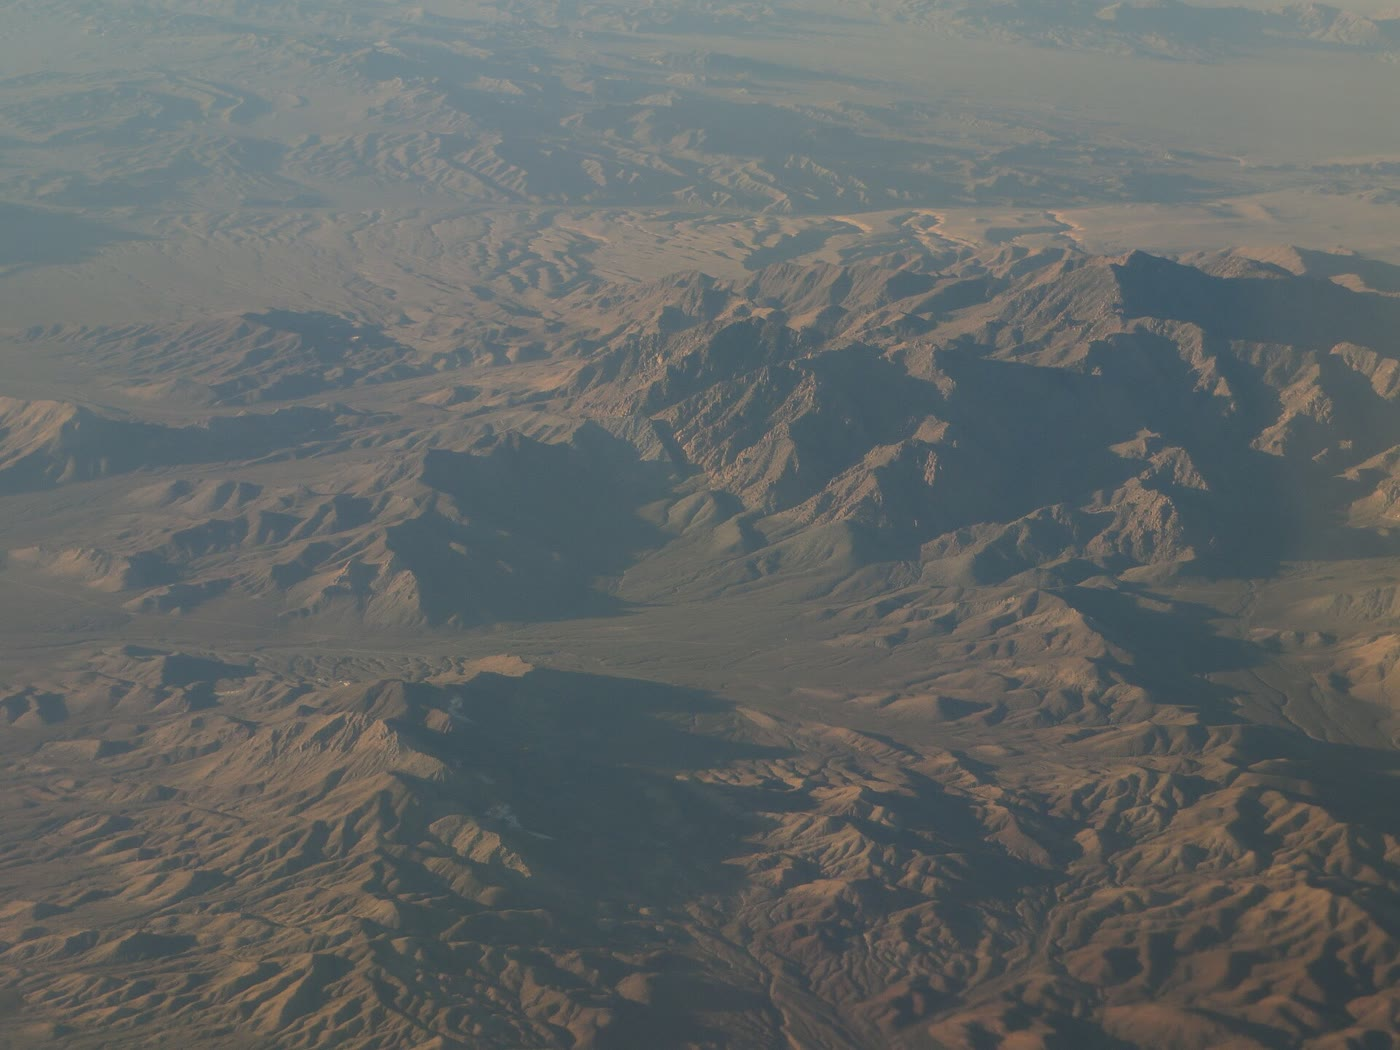
\includegraphics[width=\linewidth]{images/book5/b3-basin-and-range.jpg}

{\scriptsize Topografi basin-and-range di selatan Death Valley, California,
dari udara: pegunungan sejajar berupa blok sesar miring yang dipisahkan oleh
cekungan terisi sedimen. Foto: Ken Lund, CC BY-SA 2.0.}
\end{minipage}
\end{inthefield}
% ledger: photo:b3-basin-and-range

\section{Latihan}

\begin{exercise}[$\star$]\label{exo:b3:extension-strike-slip:1}
Suatu domain domino kaku memiliki sesar yang miring \ang{35}; sesar itu terbentuk pada
\ang{50}. Hitung kemiringan lapisan dan faktor perpanjangan.
\end{exercise}

\begin{exercise}[$\star$]\label{exo:b3:extension-strike-slip:2}
Nyatakan apakah setiap loncatan membuka cekungan atau mengangkat punggungan: sesar dekstral
yang melompat ke kanan; sesar dekstral yang melompat ke kiri; sesar sinistral yang melompat
ke kiri; sesar sinistral yang melompat ke kanan.
\end{exercise}

\begin{exercise}[$\star$]\label{exo:b3:extension-strike-slip:3}
Sesar transform Laut Mati telah bergerak \qty{105}{km} dalam sekitar \qty{20}{Ma}.
Hitung laju rata-rata dalam \unit{mm/yr} dan bandingkan dengan \qty{6}{mm/yr}
yang dipakai untuk cekungan Laut Mati.
\end{exercise}

\begin{exercise}[$\star$]\label{exo:b3:extension-strike-slip:4}
Di bagian tengah Basin and Range, perpanjangan \qty{235}{km} mencapai
\qty{200}{\percent}. Hitung lebar wilayah sebelum dan sesudah. Lakukan hal yang sama
untuk bagian utara, pada \qty{50}{\percent}.
\end{exercise}

\begin{exercise}[$\star\star$]\label{exo:b3:extension-strike-slip:5}
Sesar San Andreas telah bergerak setidaknya \qty{563}{km} dalam 15 hingga
\qty{20}{Ma}. Hitung rentang laju rata-rata, dan bandingkan dengan
pergeseran saat ini sekitar \qty{51}{mm/yr}. Apa yang bisa menjelaskan selisih tersebut?
\end{exercise}

\begin{exercise}[$\star\star$]\label{exo:b3:extension-strike-slip:6}
Dengan $\mu = 0.6$, hitung rasio $\sigma_1/\sigma_3$ yang diperlukan agar sesar normal
yang miring \ang{60}, \ang{50}, dan \ang{40} tergelincir, serta kemiringan penguncian.
\end{exercise}

\begin{exercise}[$\star\star$]\label{exo:b3:extension-strike-slip:7}
Hitung kemiringan penguncian sesar normal untuk $\mu = 0.4$ dan $\mu = 0.2$.
Koefisien gesekan berapa yang memungkinkan sesar yang miring \ang{15} tergelincir di bawah
$\sigma_1$ vertikal?
\end{exercise}

\begin{exercise}[$\star\star$]\label{exo:b3:extension-strike-slip:8}
Pada penampang seismik yang sejajar dengan gerak geser, \omterm{def:b3:extension-strike-slip:detachment}{sesar listrik} memiliki
lompatan horizontal \qty{2.5}{km}; sesar ini melandai menjadi \omterm{def:b3:extension-strike-slip:detachment}{sesar detasemen} sedalam \qty{4.0}{km}. Hitung
luas lekukan di bawah puncak awal dinding gantung, dan di bawah lapisan
pertama yang berada sedalam \qty{1.5}{km}.
\end{exercise}

\begin{exercise}[$\star\star$]\label{exo:b3:extension-strike-slip:9}
Cekungan Laut Mati memiliki panjang \qty{132}{km} dan meregang dengan faktor 1.19
sepanjang sumbunya. Hitung panjang awalnya dan besar peregangannya, serta waktu
yang dibutuhkan peregangan itu pada laju \qty{6}{mm/yr}.
\end{exercise}

\begin{exercise}[$\star\star\star$]\label{exo:b3:extension-strike-slip:10}
Blok-blok yang berjarak \qty{3.0}{km}, diukur tegak lurus terhadap sesarnya, berotasi
dari kemiringan sesar \ang{60} menjadi \ang{45}. Hitung lebar horizontal satu
blok sebelum dan sesudahnya, perpanjangan per blok, dan kemiringan lapisannya.
Mengapa lapisan harus miring ke arah yang berlawanan dengan sesarnya?
\end{exercise}

\begin{exercise}[$\star\star\star$]\label{exo:b3:extension-strike-slip:11}
Berikan sudut geser R dan R$'$ serta rekahan tarik untuk batuan dengan
$\phi = \ang{40}$ di dalam zona sinistral yang berjurus barat--timur, sebagai
azimut, beserta arah geraknya.
\end{exercise}

\begin{exercise}[$\star\star\star$]\label{exo:b3:extension-strike-slip:12}
Sebuah domain domino terbentuk dengan sesarnya pada kemiringan terbaik untuk tergelincir dan
berotasi hingga terkunci. Hitung faktor peregangan terbesar yang dihasilkan
rotasi saja untuk $\mu = 0.6$ dan untuk $\mu = 0.85$, serta sebutkan batuan mana yang
masih dapat meregang lebih jauh sebelum sesar baru harus terbentuk.
\end{exercise}

\section{Soal: Paruh-graben Merrow}

\begin{problem}[{Soal akhir pekan --- perpanjangan tepi celah rekaan,
dari domino-dominonya, sesar listriknya, kompleks inti metamorfnya dan
sesar transfernya}]
\label{pb:b3:extension-strike-slip:1}
% values: calc/ch09.py; domino_extension.py; rollover.py
Paruh-graben Merrow adalah cekungan rekaan di tepi celah benua.
Sesar utamanya berbentuk listrik dengan kemiringan \ang{60} di permukaan. Di dinding gantungnya,
sebuah domain selebar \qty{24.0}{km} dipotong oleh sesar planar yang kini miring
\ang{42} ke timur, sementara lapisan di antara sesar-sesar itu miring \ang{18} ke barat. Pada penampang seismik
yang sejajar dengan gerak geser, sesar utama memiliki lompatan horizontal \qty{3.2}{km}, dan
puncak dinding gantungnya melandai di bawah tingkat awalnya seluas
\qty{16.0}{km^2}. Ke arah selatan sepanjang jurus, erosi telah menyingkirkan lempeng atas dari
sistem yang sama dan menyingkapkan \omterm{def:b3:extension-strike-slip:core-complex}{kompleks inti metamorf}. Ke arah utara, sesar transfer sinistral
menghubungkan paruh-graben ini dengan yang berikutnya. Ambil $\mu =
0.6$, $g = \qty{9.8}{m/s^2}$ dan massa jenis kerak
\qty{2800}{kg/m^3}.

\medskip\noindent\textbf{Bagian I --- Domino-dominonya.}
\begin{enumerate}
  \item Mengapa kemiringan awal sesar sama dengan jumlah kemiringan sesar dan lapisan saat ini?
        Berikan nilainya, dan bandingkan dengan teori Anderson.
  \item Hitung faktor peregangan domain tersebut.
  \item Hitung lebar awalnya dan perpanjangan yang tercatat di dalamnya.
  \item Hitung rasio $\sigma_1/\sigma_3$ yang diperlukan agar sesar tergelincir sekarang,
        dan bandingkan dengan rasio untuk sesar baru yang berorientasi baik.
  \item Pada kemiringan berapa sesar-sesar ini terkunci, dan faktor peregangan apa yang
        dapat dicapai domain itu hanya dengan rotasi? Apa yang terjadi kemudian?
\end{enumerate}

\medskip\noindent\textbf{Bagian II --- Sesar utama listrik.}
\begin{enumerate}[resume]
  \item Jelaskan, dengan konstruksi lompatan konstan, mengapa lapisan dinding gantung
        miring ke arah sesar.
  \item Hitung kedalaman detasemennya.
  \item Luas lekukan diketahui hingga \qty{10}{\percent}. Seberapa baik
        kedalaman itu diketahui?
  \item Berapa luas lekukan yang kamu prediksi untuk lapisan yang mula-mula
        berada sedalam \qty{2.0}{km}?
  \item Berapa perpanjangan horizontal melintasi sesar utama?
  \item Bagaimana sedimen paruh-graben mencatat aktivitas
        sesar itu?
\end{enumerate}

\medskip\noindent\textbf{Bagian III --- Kompleks inti metamorf.}
\begin{enumerate}[resume]
  \item Milonit dari dinding bawah mencapai kesetimbangan pada \qty{5.5}{kbar}. Hitung
        kedalamannya.
  \item Mikanya menutup terhadap argon pada \qty{24}{Ma}, dan kerakal dari milonit yang sama
        muncul di dalam isian paruh-graben pada \qty{16}{Ma}. Hitung
        laju ekshumasi rata-rata, dengan menganggap kedalaman penutupan sebagai kedalaman
        pada pertanyaan sebelumnya.
  \item Untuk membawa milonit ke atas, berapa besar pergeseran yang diperlukan pada detasemen
        dengan kemiringan rata-rata \ang{30}, dan berapa perpanjangan horizontalnya?
  \item Detasemen itu miring \ang{15} di permukaan saat ini. Mungkinkah ia tergelincir pada kemiringan itu di bawah
        $\sigma_1$ vertikal? Berikan dua jalan keluar.
  \item Jika ia tergelincir pada \ang{45} di kedalaman, bagian yang tersingkap
        berotasi melalui sudut berapa, dan mengapa?
  \item Bandingkan perpanjangan kompleks inti dengan perpanjangan
        paruh-graben.
\end{enumerate}

\medskip\noindent\textbf{Bagian IV --- Sesar transfer.}
\begin{enumerate}[resume]
  \item Sesar transfer sinistral bergeser ke kiri sejauh \qty{4.0}{km}, dengan kedua untaiannya
        saling tumpang tindih sepanjang \qty{3.0}{km}. Apakah langkah itu membuka cekungan
        atau mengangkat punggungan?
  \item Sesar itu bergeser pada \qty{5}{mm/yr} selama \qty{1.2}{Ma}. Hitung
        besar pergeserannya.
  \item Hitung luas yang terbuka, panjang dasar cekungan (tumpang tindih ditambah
        pergeseran), dan rasio panjang terhadap lebarnya.
  \item Bandingkan rasio itu dengan rasio Cekungan Laut Mati, yang panjangnya \qty{132}{km} dan
        lebarnya 7 hingga \qty{10}{km}.
  \item Di tempat sesar yang sama membelok ke arah sebaliknya, struktur apa yang terbentuk, dan
        apa yang akan ditunjukkan oleh penampang melintang yang melewatinya?
  \item Berapa total perpanjangan horizontal melintasi paruh-graben Merrow,
        dari sesar utamanya dan domino-dominonya?
\end{enumerate}
\end{problem}
